\documentclass{article}
\usepackage[utf8]{inputenc}
\usepackage{graphicx}
\usepackage{amsmath}
\usepackage{amssymb}
\usepackage{subfig}
\usepackage{listings}
\usepackage{algorithm}
\usepackage{algorithmic}
\usepackage{caption}
\usepackage{tikz}
\usepackage{url}
\usetikzlibrary{arrows.meta,fit,positioning}

\title{Machine Learning with Graphs:\\ Homework 4 - Graph Embedding and Graphical Models}
\author{}
\date{Spring 2026}

\begin{document}

\maketitle

This submission solves Problems 1 and 2.

\section*{Problem 1 (conceptual)}

Consider the graphical model shown in Figure \ref{fig::p1}.

\paragraph{a)} One reasonable interpretation is \emph{quality control in a manufacturing line}. The left part of the graph describes the quality of the motherboard subsystem, the right part describes the quality of the battery/thermal subsystem, and the bottom node is the final burn-in test. A concrete mapping is:
\begin{itemize}
    \item $x_2$: quality of the incoming electronic components,
    \item $x_3$: precision of the soldering/calibration process,
    \item $x_1$: observed early electrical test result,
    \item $x_4$: latent quality of the motherboard subsystem,
    \item $x_7$: quality of the battery cells,
    \item $x_8$: quality of the thermal assembly process,
    \item $x_9$: observed battery diagnostics reading,
    \item $x_6$: latent health of the battery/thermal subsystem,
    \item $x_5$: observed final burn-in test result.
\end{itemize}
In this interpretation, better components and better soldering influence both the early electrical test ($x_1$) and the true motherboard quality ($x_4$). Similarly, battery-cell quality and thermal assembly quality influence both the battery diagnostics reading ($x_9$) and the true battery/thermal health ($x_6$). The final burn-in result ($x_5$) depends on both subsystems.

\newcommand{\bigCI}{\mathrel{\text{\scalebox{1.07}{$\perp\mkern-10mu\perp$}}}}

\paragraph{b)} I interpret the independence questions using d-separation on the underlying DAG structure. Under that interpretation:
\begin{center}
\small
\renewcommand{\arraystretch}{1.25}
\begin{tabular}{|p{0.22\linewidth}|c|p{0.58\linewidth}|}
\hline
\textbf{Statement} & \textbf{Answer} & \textbf{Reason} \\
\hline
\(x_1 \bigCI x_4\) & NO & \(x_1 \leftarrow x_2 \rightarrow x_4\) is an open path. \\
\hline
\(x_2 \bigCI x_3\) & YES & \(x_2 \rightarrow x_1 \leftarrow x_3\) and \(x_2 \rightarrow x_4 \leftarrow x_3\) are both colliders. \\
\hline
\(x_2 \bigCI x_7\) & YES & Every path from \(x_2\) to \(x_7\) goes through the collider \(x_5\). \\
\hline
\(x_1 \bigCI x_4 \mid x_2\) & NO & Even after conditioning on \(x_2\), the path \(x_1 \leftarrow x_3 \rightarrow x_4\) remains open. \\
\hline
\(x_2 \bigCI x_3 \mid x_1\) & NO & Conditioning on the collider \(x_1\) opens the path \(x_2 \rightarrow x_1 \leftarrow x_3\). \\
\hline
\(x_2 \bigCI x_7 \mid x_5\) & NO & Conditioning on the collider \(x_5\) opens \(x_2 \rightarrow x_4 \rightarrow x_5 \leftarrow x_6 \leftarrow x_7\). \\
\hline
\end{tabular}
\end{center}
If the shaded nodes are treated as already observed evidence, then the second and third answers also become NO because observing the colliders $x_1$ and $x_5$ opens those paths.

\paragraph{c)} All three quantities can be computed exactly with sum-product after converting the Bayesian network into an equivalent tree-structured junction tree. A convenient clique tree is
\[
\{x_1,x_2,x_3\}
\;-\;
\{x_2,x_3,x_4\}
\;-\;
\{x_4,x_5,x_6\}
\;-\;
\{x_6,x_7,x_8\}
\;-\;
\{x_7,x_8,x_9\}.
\]
From this tree:
\begin{itemize}
    \item $p(x_4)$ is available directly from a clique containing $x_4$,
    \item $p(x_4,x_6)$ is available directly from the clique $\{x_4,x_5,x_6\}$,
    \item $p(x_2,x_7)$ can also be obtained by clustering the middle part of the junction tree into a larger equivalent clique (for example, merging the middle three cliques into one super-node), then running sum-product on the resulting tree.
\end{itemize}
So the correct conclusion is that \emph{all three are computable}; the difference is computational cost, since $p(x_2,x_7)$ requires a larger cluster than the other two.

\begin{figure}[ht!]
\centerline{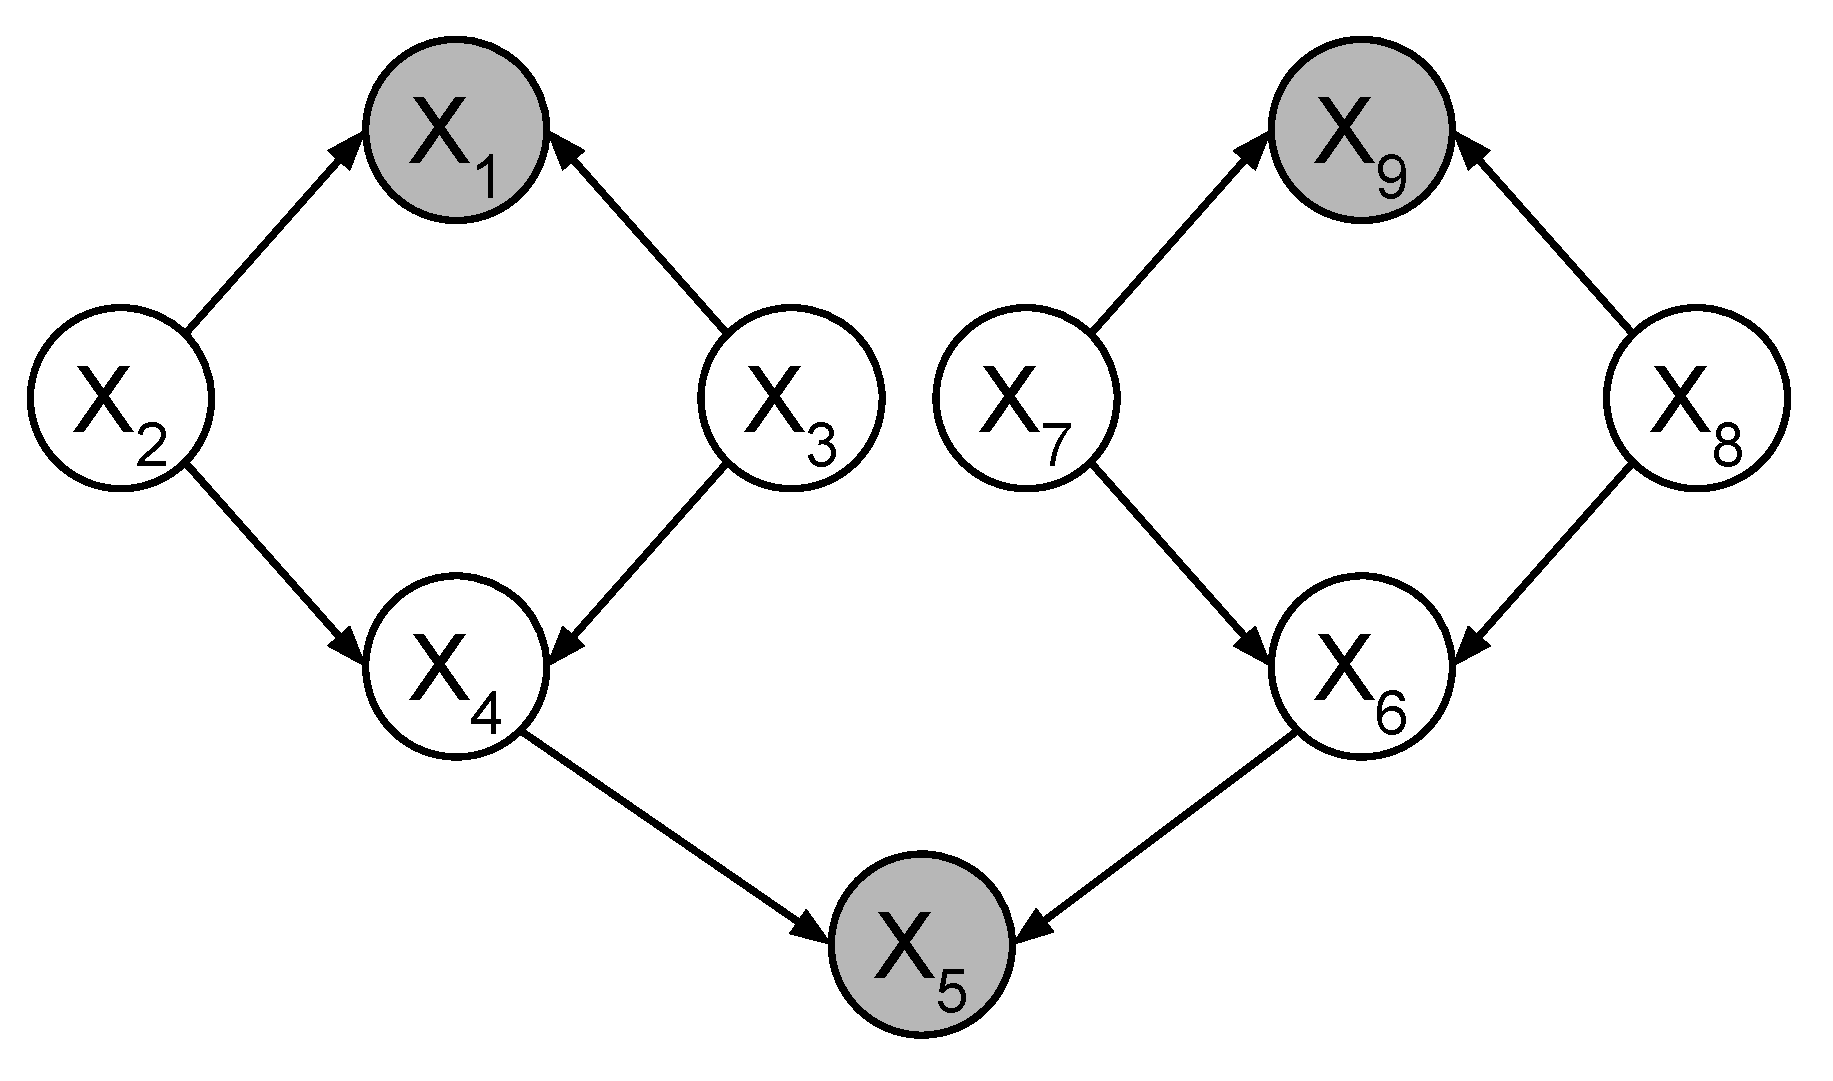
\includegraphics[width=0.7\columnwidth]{figures/hw-gm}}
\caption{Graphical model for problem 1. Only gray nodes are observed. \label{fig::p1}}
\end{figure}

\section*{Problem 2 (optional, analytical)}

\paragraph{Notation.} To represent the ``frozen'' processes explicitly, let $X_t^{(m)}$ be the hidden state of process $m$ at time $t$, for $m=1,\ldots,M$. Only the active process selected by $Z_t$ is allowed to change at time $t$.

\paragraph{a)} A natural example is a \emph{multi-speaker conversation transcript}. Suppose there are $M$ speakers. Each speaker has a private latent discourse state (for example, asking a question, giving background, answering, or making a joke) that evolves as a Markov chain. At each time step, exactly one speaker talks, so $Z_t$ identifies the active speaker. The active speaker updates their discourse state and emits the next observed word or token $Y_t$, while the latent states of the other speakers stay unchanged until they speak again.

\paragraph{b)} A two-slice dynamic Bayesian network for the extended HMM is shown in Figure \ref{fig::p2}. The plate over $m$ indicates that the same transition structure is repeated for each of the $M$ concurrent processes.

\begin{figure}[ht!]
\centering
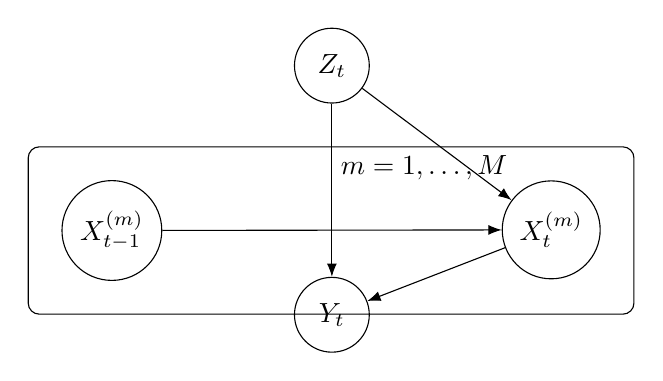
\begin{tikzpicture}[>=Latex, node distance=1.6cm]
    \tikzstyle{rv}=[circle,draw,minimum size=0.95cm]
    \node[rv] (z) {$Z_t$};
    \node[rv, below left=1.3cm and 2.0cm of z] (xprev) {$X_{t-1}^{(m)}$};
    \node[rv, below right=1.3cm and 2.0cm of z] (xcur) {$X_t^{(m)}$};
    \node[rv, below=2.2cm of z] (y) {$Y_t$};

    \draw[->] (xprev) -- (xcur);
    \draw[->] (z) -- (xcur);
    \draw[->] (z) -- (y);
    \draw[->] (xcur) -- (y);

    \node[draw,rounded corners,fit=(xprev) (xcur),inner sep=12pt,label={[below right]{$m=1,\ldots,M$}}] {};
\end{tikzpicture}
\caption{Two-slice DBN for the extended HMM. The plate means there are $M$ chains $X_t^{(1)},\ldots,X_t^{(M)}$. The CPD of $Y_t$ uses $Z_t$ to select the currently active hidden chain.}
\label{fig::p2}
\end{figure}

\paragraph{c)} Let $\mathbf{X}^{(m)} = (X_1^{(m)},\ldots,X_T^{(m)})$ be the state sequence of process $m$. The joint distribution can be written as
\begin{align*}
p(\mathbf{y},\mathbf{z},\mathbf{x}^{(1)},\ldots,\mathbf{x}^{(M)})
&=
\left(\prod_{m=1}^{M} p(x_1^{(m)})\right)
\left(\prod_{t=1}^{T} p(z_t)\right)
\left(\prod_{t=1}^{T} p(y_t \mid z_t, x_t^{(1)},\ldots,x_t^{(M)})\right) \\
&\qquad \times
\left(\prod_{t=2}^{T} \prod_{m=1}^{M} p(x_t^{(m)} \mid x_{t-1}^{(m)}, z_t)\right),
\end{align*}
where $p(z_t=m)=c_m$, and the transition term is
\[
p(x_t^{(m)} \mid x_{t-1}^{(m)}, z_t)
=
\begin{cases}
A^{(m)}\!\left(x_t^{(m)} \mid x_{t-1}^{(m)}\right), & z_t=m,\\[4pt]
\mathbb{I}\!\left[x_t^{(m)} = x_{t-1}^{(m)}\right], & z_t\neq m,
\end{cases}
\]
so only the selected chain evolves. The emission term uses the active chain:
\[
p(y_t \mid z_t, x_t^{(1)},\ldots,x_t^{(M)})
=
B^{(z_t)}\!\left(y_t \mid x_t^{(z_t)}\right).
\]

\paragraph{d)} The standard conversion is to build one \emph{super-state} that stores all information needed to make the process first-order Markov:
\[
S_t = \left(Z_t, X_t^{(1)}, X_t^{(2)}, \ldots, X_t^{(M)}\right).
\]
Then an equivalent ordinary HMM is obtained as follows:
\begin{enumerate}
    \item Define one HMM state for every possible value of $S_t$.
    \item The transition probability from $S_{t-1}$ to $S_t$ first chooses the active process $Z_t$ using $c_m$, then updates only the corresponding component $X_t^{(Z_t)}$ using that process's Markov transition matrix, while all other components remain unchanged.
    \item The emission probability of the HMM state $S_t$ is exactly the symbol distribution produced by the active process, namely $p(y_t \mid S_t)=B^{(Z_t)}(y_t \mid X_t^{(Z_t)})$.
\end{enumerate}
If every process has $K$ possible hidden states, then the equivalent HMM has
\[
M K^M
\]
hidden states. More generally, if process $m$ has $K_m$ states, the count is
\[
M\prod_{m=1}^{M} K_m.
\]
This construction is exact, but I would \emph{not} claim it is always minimum: unreachable states or parameter symmetries can sometimes be merged, so $M K^M$ is best viewed as a clean upper bound for a standard HMM representation.


\end{document}
